\section{The role of the \texorpdfstring{$\alpha$}{TEXT} coefficient in the intensity function}\label{app:role_alpha_coef}

Here we seek to determine an intuitive approach to the role of the coefficient $\alpha$ in intensity, Eq.~\eqref{eq:intensity_definition}.
The goal of this approach is to determine a function that will allow to initialize the $\alpha$ parameter for the EM algorithm, for the \textit{smart init}, as it has been done for the $\mu$ coefficient of the baseline.
The starting point is the Algorithm~\ref{algo:1d_inhomogenous_pp}, which allows us to simulate a non-homogenous Poisson process using a given intensity function.
The coefficient $\alpha$ intervenes at two places in this algorithm: when determining $\Bar{\lambda} = \max_{0 \leq t} \lambda(t)$, and upon acceptance, or not, of the points $s_{m+1}$.

As previously mentioned in Eq.~\eqref{eq:max_lambda}, $\Bar{\lambda} = \mu_k + \alpha_{k,p}\kappa_{k,p}\pars{m_{k,p}}$, thus, the greater the $\alpha$ coefficient, the higher the maximum intensity over the $\intervalleFF{0}{T}$ interval.
For the selected points $s_{m+1}$, two cases are to be considered: when the points are on the baseline and when the points are on the supports of the different kernels.
For more clarity, let us note the set of the supports of the various kernels $\mathcal{S}_{p}$.:
\begin{equation}
    \mathcal{S}_{p} \coloneqq \bigcup_{i = 1,\dots,n_p} \intervalleFF{t^{(p)}_i + a}{t^{(p)}_i + b}
\end{equation}

In case a selected point $s_{m+1}$ is on the baseline, i.e., $s_{m+1} \in \intervalleFF{0}{T} \setminus \mathcal{S}_{p}$, the probability to accept this point is equal to $\lambda\pars{s_{m+1}} / \Bar{\lambda} = \mu_k / \Bar{\lambda}$, and thus decreases when $\alpha$ increases.
Therefore, as $\alpha$ increases, the proportion of activations on the baseline decreases, and conversely, the proportion of activations on the kernel supports, i.e., in $\mathcal{S}_{p}$ is greater.
This relationship between the value of $\alpha$ and the proportion of activations in $\mathcal{S}_{p}$ is represented in Figure~\ref{fig:ppt_in_support}, where for each value of the coefficient $\alpha$, from 0 to 5 with a step of 0.1, the said proportion is calculated on the ordinate as follows:
\begin{equation}
    p_a \coloneqq \frac{\#\enstq{t\in\mathcal{A}_{k,p}}{t\in\mathcal{S}_{p}}}{\# \mathcal{A}_k}
\end{equation}

\begin{figure}[h!]
    \centering
    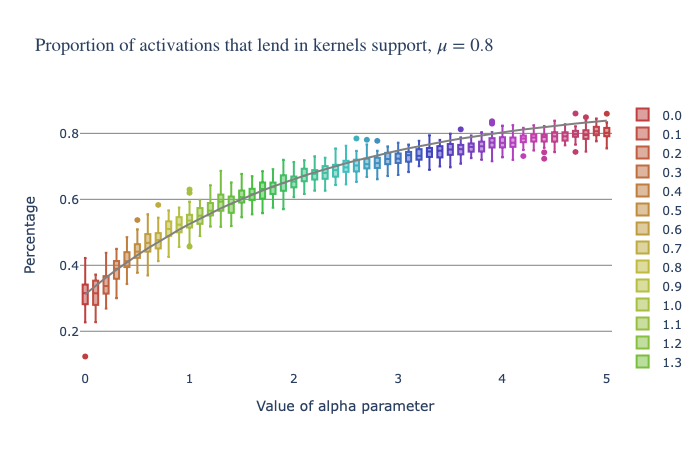
\includegraphics[scale=0.6]{pics/ppt_in_support_transp.png}
    \caption{Proportion of generated activations within $\mathcal{S}$ based on the $\alpha$ parameter, where $\mu=0.8, T=180, n_p=73, \intervalleFF{a}{b}=\bracks{30, 800} \num{e-3}$, with 50 simulations for each value of $\alpha$. In black, the function $f^{-1}(p_a)$.}
    \label{fig:ppt_in_support}
\end{figure}

As mentioned before, we are looking for a function, which, from the data, would allow us to have a first estimate of $\alpha$, in order to initialise the EM algorithm intuitively.
A first observation that can be made with the help of this figure is that there is most probably a relationship between the value of the coefficient $\alpha$ and $p_a$.
If we manage to establish such a relation, then, by taking its inverse, we will be able to determine a first value of $\alpha$ from the proportion $p_a$, which can be calculated immediately from the data.
We can then initiate $\alpha$ in the following way:
\begin{equation}
    \alpha^{(0)} = f(p_a)
\end{equation}

A first observation that can be made from the outset is that, whatever the values of the parameters, $\alpha$, $\mu$, $T$, etc., $p_a$ will always be below 1, by definition.
So, looking at the shape of the relationship in Figure~\ref{fig:ppt_in_support}, a first idea is the following:
\begin{equation}\label{eq:alpha_init_1}
    f(p_a) = -\ln \pars{1-p_a}
\end{equation}

When $\alpha = 0$, the intensity is reduced to its baseline, i.e., $\lambda_{k,p}(t) = \mu_k, \forall t \in \intervalleFF{0}{T}$, the proportion of acceptance in the simulation algorithm is therefore 1.
Thus, we find ourselves in the simple case of a simulation of a homogeneous Poisson process, i.e., with constant intensity.
Thus, the proportion of activations found in the supports of the different kernels must be simply equal to the proportion represented by all the supports in the total duration.
We note this proportion $p_s$:
\begin{equation}
    p_s \coloneqq \frac{n_p \pars{b-a}}{T}
\end{equation}

Replacing with the numerical values used for the Figure~\ref{fig:ppt_in_support} gives $p_s = 0.31$, which is consistent with the median obtained for $\alpha = 0$.

Thus, a second observation that can be made is that if $\alpha$ is always positive, then $p_a$ is always higher than $p_s$.
We then modify \ref{eq:alpha_init_1} accordingly:
\begin{equation}
    f(p_a) = -\ln\pars{1-p_a} + \ln\pars{1-p_s} = -\ln\pars{\frac{1 - p_a}{1 - p_s}}
\end{equation}

In addition, the stronger the baseline, the less $p_a$ increases, so we want the curvature to decrease when $\mu$ increases:
\begin{equation}
    f(p_a) = - e^{\mu} \ln\pars{\frac{1 - p_a}{1 - p_s}}
\end{equation}

Likewise, the higher $\mu$ is, the harder it is for $p_a$ to reach the limit of 1.
However, we do not consider values of $\alpha$ too high, in order to remain realistic, and so we especially want a good estimate of $\alpha$ for values lower than 5.
Therefore, we propose to adapt the limit according to $\mu$:
\begin{equation}
    f(p_a) = - e^{\mu} \ln\pars{\frac{l(\mu) - p_a}{l(\mu)  - p_s}}
\end{equation}
where $l(\mu)$ is a function which is worth 1 when $\mu = 0$ (in this case all the activations are in $\mathcal{S}$, $p_a = 1$), and which tends towards $p_s$ when $\mu$ increases (because we recall that $p_a$ cannot be systematically lower than $p_s$ for positive values of $\alpha$).

Thus, we propose:
\begin{equation}
    l(\mu) = \pars{\frac{e^{\mu}-1}{5} + \frac{1}{1-p_s}}^{-1} + p_s
\end{equation}

In order to test our initialisation function, and to show that it is better than chance, we calculate $\alpha^{(0)} = f(p_a)$, for different values of $\mu$ and $\alpha$, for 50 simulations each time.
The RMSE (\textit{Root Mean Square Error}) is then calculated.
The result is shown in Figure~\ref{fig:heatmap_alpha_init_rmse}.

\begin{figure}[h!]
    \centering
    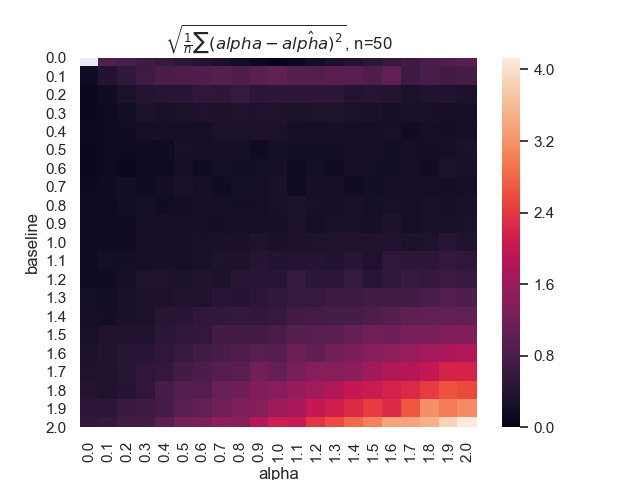
\includegraphics[scale=0.7]{pics/heatmap_baseline_alpha_alpha_init_rmse.jpg}
    \caption{RMSE between the calculated value for $\alpha^{(0)}$ and its true value, for different values of $\mu$ and $\alpha$.}
    \label{fig:heatmap_alpha_init_rmse}
\end{figure}

It can be seen from this figure that the estimate made of $\alpha$ is more than correct (i.e., cases where the RMSE is smaller than 1) in two main situations\footnote{We do not take into account the degenerate case where $\mu = \alpha = $0.}:
\begin{itemize}
    \item when the $\mu$ baseline is low, but greater than 0.2, for all values of $\alpha$; 
    \item when the $\alpha$ coefficient is low for all values in the baseline.
\end{itemize}

Conversely, the more $\mu$ and $\alpha$ increase simultaneously, the less accurate the initial estimate of $\alpha$ is.

There is a second degenerate case, in addition to the case where $\mu = \alpha = 0$: when $\mu = 0$ and $\alpha > 0$.
In this case, since the baseline is null, all activations are present on the kernel supports, because in the Algorithm~\ref{algo:1d_inhomogenous_pp}, if $s_{m+1} \notin \mathcal{S}$, then the intensity is null and therefore the probability of accepting such a point is also null.
Thus, we have $p_a = 1$, and $l(\mu) = 1$, and then $f(p_a)$ is worth $+\infty$.
So, when one is in this situation, one decides to return 1:
\begin{equation}
    f(p_a ; \mu, p_s) = 
    \left\{
		\begin{array}{ll}
			f(p_a) & \mbox{si } \mu > 0 \text{ ou } p_a > 0 \\
			1 & \mbox{sinon}
		\end{array}
	\right.
\end{equation}

\paragraph{Remark} In practice, the $\mu$ parameter of the function $f(p_a; \mu, p_s)$ is not the true value of the baseline, but the calculated value for its initialisation, as defined in Eq.~\eqref{eq:baseline_init}.


